\documentclass[preview, border=8pt, multi, tikz]{standalone}
\usepackage{tikz}
\usepackage{import}
\subimport{./layers/}{init}
\usetikzlibrary{positioning}
\usetikzlibrary{3d} %for including external image
\def\ConvColor{rgb:yellow,5;red,2.5;white,5}
\def\ConvReluColor{rgb:yellow,5;red,5;white,5}
\def\PoolColor{rgb:red,1;black,0.3}
\def\UnpoolColor{rgb:blue,2;green,1;black,0.3}
\def\FcColor{rgb:blue,5;red,2.5;white,5}
\def\FcReluColor{rgb:blue,5;red,5;white,4}
\def\SoftmaxColor{rgb:magenta,5;black,7}


\newcommand{\copymidarrow}{\tikz \draw[-Stealth,line width =0.8mm,draw={rgb:blue,4;red,1;green,1;black,3}] (-0.3,0) -- ++(0.3,0);}

\begin{document}
\begin{tikzpicture}
\tikzstyle{connection}=[ultra thick,every node/.style={sloped,allow upside down},draw=\edgecolor,opacity=0.7]

\tikzstyle{copyconnection}=[ultra thick,every node/.style={sloped,allow upside down},draw={rgb:blue,4;red,1;green,1;black,3},opacity=0.7]

\node[canvas is zy plane at x=0] (temp) at (-1.75,0,0) {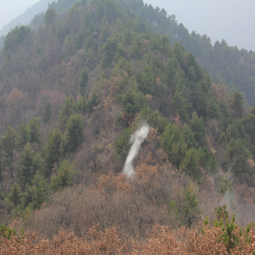
\includegraphics[width=8.5cm,height=8.5cm]{image.png}};
%%%%%%%%%%%%%%%%%%%%%%%%%%%%%%%%%%%%%%%%%%%%%%%%%%%%%%%%%%%%%%%%%%%%%%%%%%%%%%%%%%%%%%%%
%% Draw Encoder
%%%%%%%%%%%%%%%%%%%%%%%%%%%%%%%%%%%%%%%%%%%%%%%%%%%%%%%%%%%%%%%%%%%%%%%%%%%%%%%%%%%%%%%%

% down11, down12
\pic[shift={(0,0,0)}] at (0,0,0) {Box={name=down1,%
        xlabel={{"64", "64"}},zlabel = I, fill=\ConvColor,%
        height=40,width={2,2},depth=40}};
%%%%%%%%%%
% down21, down22
\pic[shift={(3,-5,0)}] at (down1-south) 
{Box={name=down2,%
        xlabel={{"128","128"}},zlabel=I/2,fill=\ConvColor,%
        height=32,width={4,4},depth=32}};
%%%%%%%%%%
% down31, down32
\pic[shift={(2,-5,0)}] at (down2-south) 
{Box={name=down3,%
        xlabel={{"256","256"}},zlabel=I/4,fill=\ConvColor,%
        height=25,width={8,8},depth=25}};
%%%%%%%%%%
% down41, down42
\pic[shift={(2,-6,0)}] at (down3-east)
{Box={name=down4,%
        xlabel={{"512","512"}},zlabel=I/8,fill=\ConvColor,%
        height=16,width={16,16},depth=16}};
%%%%%%%%%%%%%%%%%%%%%%%%%%%%%%%%%%%%%%%%%%%%%%%%%%%%%%%%%%%%%%%%%%%%%%%%%%%%%%%%%%%%%%%%
%% Bottleneck
%%%%%%%%%%%%%%%%%%%%%%%%%%%%%%%%%%%%%%%%%%%%%%%%%%%%%%%%%%%%%%%%%%%%%%%%%%%%%%%%%%%%%%%%% bottle neck
\pic[shift={(2,-4,0)}] at (down4-south) {Box={name=bottle,caption=BottleNeck,%
        xlabel={{"1024", "dummy"}},zlabel=I/16,fill=\ConvColor,%
        height=8,width={32},depth=8}};
%%%%%%%%%%%%%%%%%%%%%%%%%%%%%%%%%%%%%%%%%%%%%%%%%%%%%%%%%%%%%%%%%%%%%%%%%%%%%%%%%%%%%%%%
%% Draw Decoder 
%%%%%%%%%%%%%%%%%%%%%%%%%%%%%%%%%%%%%%%%%%%%%%%%%%%%%%%%%%%%%%%%%%%%%%%%%%%%%%%%%%%%%%%%
%% up4, 
\pic[shift={(5, 0, 0)}] at (down4-east)
{Box={name=cat4,%
        xlabel = {{"512", "dummy"}}, fill=\UnpoolColor,
        height=16,width=16,depth=16}};
\pic[shift={(0,0,0)}] at (cat4-east)
{Box={name=up4,%
        xlabel={{"512", "dummy"}},fill=\ConvColor,%
        height=16,width=16,depth=16}};
\pic[shift={(2,0,0)}] at (up4-east) 
{Box={name=upconv4,%
        xlabel={{"512","512"}},fill=\ConvColor,
        height=16,width={16, 16},depth=16}};    
%%%%%%%%%%
%% up3, 
\pic[shift={(30,0,0)}] at (down3-east)
{Box={name=cat3,%
        xlabel = {{"256", "dummy"}}, fill=\UnpoolColor,height=25,width=8,depth=25}};
\pic[shift={(0,0,0)}] at (cat3-east)
{Box={name=up3,%
        xlabel={{"256", "dummy"}},fill=\ConvColor,%
        height=25,width=8,depth=25}};
\pic[shift={(2,0,0)}] at (up3-east) 
{Box={name=upconv3,%
        xlabel={{"256","256"}}, zlabel = I/8, fill=\ConvColor,
        height=25,width={8, 8},depth=25}}; 
%%%%%%%%%%
%% up2, 
\pic[shift={(48,0,0)}] at (down2-east)
{Box={name=cat2,%
        xlabel = {{"128", "dummy"}}, fill=\UnpoolColor,height=32,width=4,depth=32}};
\pic[shift={(0,0,0)}] at (cat2-east)
{Box={name=up2,%
        xlabel={{"128", "dummy"}},fill=\ConvColor,%
        height=32,width=4,depth=32}};
\pic[shift={(2,0,0)}] at (up2-east) 
{Box={name=upconv2,%
        xlabel={{"128","128"}}, zlabel = I/2, fill=\ConvColor,
        height=32,width={4, 4},depth=32}}; 
%%%%%%%%%%
%% up1, 
\pic[shift={(60,0,0)}] at (down1-east)
{Box={name=cat1,%
        xlabel = {{"64", "dummy"}}, fill=\UnpoolColor,height=40,width=2,depth=40}};
\pic[shift={(0,0,0)}] at (cat1-east)
{Box={name=up1,%
        xlabel={{"64", "dummy"}},fill=\ConvColor,%
        height=40,width=2,depth=40}};
\pic[shift={(2,0,0)}] at (up1-east) 
{Box={name=upconv1,%
        xlabel={{"64","64"}}, zlabel = I, fill=\ConvColor,
        height=40,width={2, 2},depth=40}}; 
\pic[shift={(2,0,0)}] at (upconv1-east) 
{Box={name=finalconv,%
        xlabel={{"2","dummy"}}, zlabel = I, fill=\ConvColor,
        height=40,width={0.5, 0.5},depth=40}};
%%%%%%%%%%%%%%%%%%%%%%%%%%%%%%%%%%%%%%%%%%%%%%%%%%%%%%%%%%%%%%%%%%%%%%%%%%%%%%%%%%%%%%%%
%% final
%%%%%%%%%%%%%%%%%%%%%%%%%%%%%%%%%%%%%%%%%%%%%%%%%%%%%%%%%%%%%%%%%%%%%%%%%%%%%%%%%%%%%%%%%
% \pic[shift={(0.75,0,0)}] at (upconv1-east) 
% {Box={name=upconv0,%
%         xlabel={{"1","1"}}, zlabel = img_size, fill=\ConvColor,
%         height=40,width={2, 2},depth=40}}; 
        
\node[canvas is zy plane at x=0] (temp) at (70,0,0) {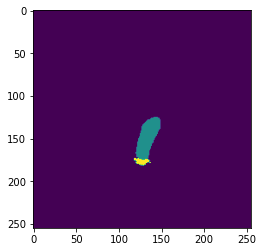
\includegraphics[width=10cm,height=10cm]{mask.png}};

%\pic[shift={(0.75,0,0)}] at (ucr1a-east) {Box={name=out,caption=Softmax,
%        zlabel=I,fill=\SoftmaxColor,height=40,width=1,depth=40}};
%%%%%%%%%%%%%%%%%%%%%%%%%%%%%%%%%%%%%%%%%%%%%%%%%%%%%%%%%%%%%%%%%%%%%%%%%%%%%%%%%%%%%%%
% Draw connections
%%%%%%%%%%%%%%%%%%%%%%%%%%%%%%%%%%%%%%%%%%%%%%%%%%%%%%%%%%%%%%%%%%%%%%%%%%%%%%%%%%%%%%%
\path (down4-north) -- (down4-south) coordinate[pos=2.25] (down4-bot);
\path (down3-north) -- (down3-south) coordinate[pos=1.7] (down3-bot);
\path (down2-north) -- (down2-south) coordinate[pos=1.775] (down2-bot);
\path (down1-north) -- (down1-south) coordinate[pos=1.625] (down1-bot);

\path (up4-north) -- (up4-south) coordinate[pos=2.25] (up4-bot);
\path (up3-north) -- (up3-south) coordinate[pos=1.7] (up3-bot);
\path (up2-north) -- (up2-south) coordinate[pos=1.775] (up2-bot);
\path (up1-north) -- (up1-south) coordinate[pos=1.625] (up1-bot);

\draw [connection]  (down1-south)
--node{\copymidarrow}(down1-bot)
--node{\copymidarrow}(down2-west);
\draw [connection]  (down2-south)
--node{\copymidarrow}(down2-bot)
--node{\copymidarrow}(down3-west);
\draw [connection]  (down3-south)
--node{\copymidarrow}(down3-bot)
--node{\copymidarrow}(down4-west);
\draw [connection]  (down4-south)
--node {\copymidarrow} (down4-bot)
-- node {\midarrow} (bottle-west);
%%%%%%%%%
\draw [connection]  (bottle-east)  
--node{\copymidarrow upConv 2x2}(up4-bot)
--node{\midarrow upConv 2x2} (up4-south);
\draw [connection]  (upconv4-east)  
--node{\copymidarrow upConv 2x2}(up3-bot)
--node{\midarrow upConv 2x2} (up3-south);
\draw [connection]  (upconv3-east)  
--node{\copymidarrow upConv 2x2}(up2-bot)
--node{\midarrow upConv 2x2} (up2-south);
\draw [connection]  (upconv2-east)  
--node{\copymidarrow upConv 2x2}(up1-bot)
--node{\midarrow upConv 2x2} (up1-south);
%%%%%%%%%
\draw [connection]  (up4-east)  -- node {\midarrow doubleConv, ReLU} (upconv4-west);
\draw [connection]  (up3-east)  -- node {\midarrow doubleConv, ReLU} (upconv3-west);
\draw [connection]  (up2-east)  -- node {\midarrow doubleConv, ReLU} (upconv2-west);
\draw [connection]  (up1-east)  -- node {\midarrow doubleConv, ReLU} (upconv1-west);
\draw [connection] (upconv1-east) --node{\midarrow Conv 1x1} (finalconv-west);

% %%%%
\draw [connection]  (down4-east)  
-- node {\midarrow skip connection} (cat4-west);
\draw [connection]  (down3-east) 
-- node {\midarrow skip connection} (cat3-west);
\draw [connection]  (down2-east) 
-- node {\midarrow skip connection} (cat2-west);
\draw [connection]  (down1-east) 
-- node {\midarrow skip connection} (cat1-west);
%%%%%%%%%%%%%%%%%%%%%%%%%%%%%%%%%%%%%%%%%%%%%%%%%%%%%%%%%%%%%%%%%%%%%%%%%%%%%%%%%%%%%%%
\end{tikzpicture}
\end{document}